\documentclass[border=5pt]{standalone}
\usepackage[dvipsnames]{xcolor}
\usepackage{tikz}
\usetikzlibrary{arrows.meta,positioning,shapes.geometric,calc,fit,decorations.pathreplacing}
\usepackage{amssymb}

\definecolor{cObserve}{HTML}{2979FF}
\definecolor{cOrient}{HTML}{FF8F00}
\definecolor{cDecide}{HTML}{2E7D32}
\definecolor{cAct}{HTML}{C62828}
\definecolor{cAuto}{HTML}{7B1FA2}
\definecolor{cGray}{HTML}{616161}

\begin{document}
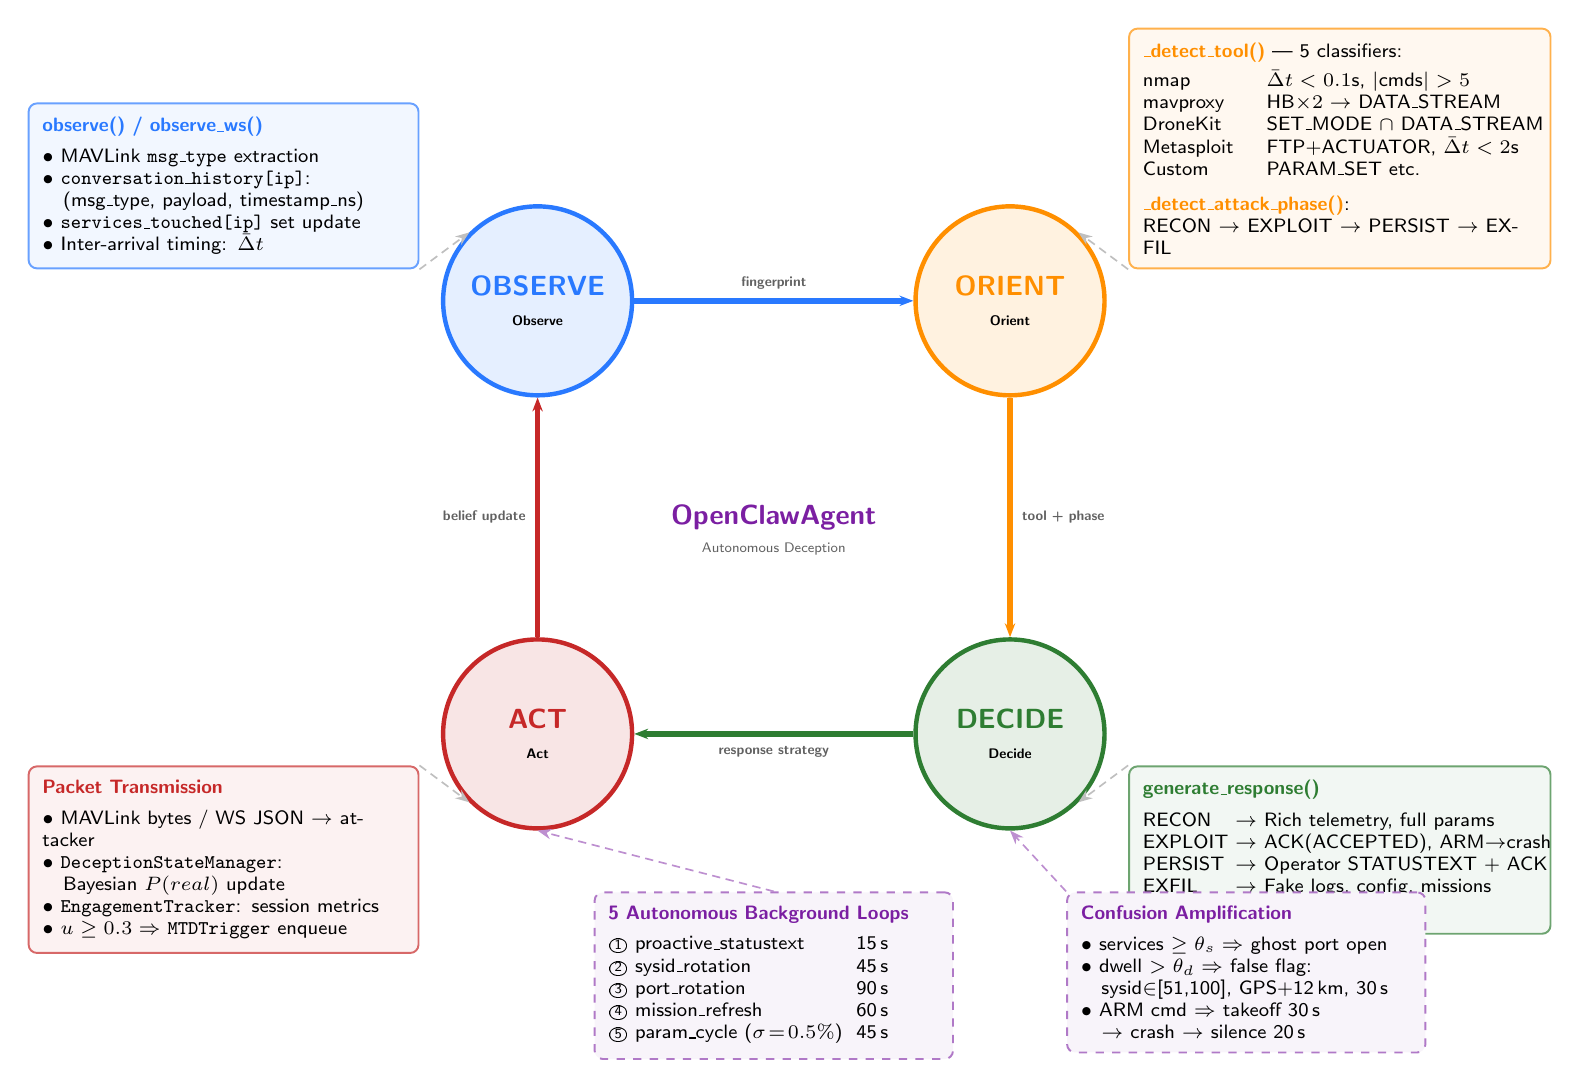
\begin{tikzpicture}[
  >={Stealth[length=5pt]},
  font=\sffamily,
  phase/.style 2 args={
    circle, draw=#1, fill=#1!12, line width=1.6pt,
    minimum size=2.4cm, align=center, font=\sffamily\bfseries
  },
  detailbox/.style 2 args={
    rectangle, rounded corners=3pt, draw=#1!70, fill=#1!6,
    line width=0.7pt, align=left, font=\sffamily\scriptsize,
    text width=#2, inner sep=5pt
  },
  autobox/.style={
    rectangle, rounded corners=3pt, draw=cAuto!60, fill=cAuto!5,
    line width=0.7pt, dashed, align=left, font=\sffamily\scriptsize,
    text width=4.2cm, inner sep=5pt
  },
  mainflow/.style={->, line width=2pt, draw=cGray},
  subflow/.style={->, line width=0.6pt, draw=gray!50, densely dashed},
]

% ════════════════════════════════════════════════════
% OODA 4 phases — diamond layout
% ════════════════════════════════════════════════════
\node[phase={cObserve}{12}] (O) at (0,0)
  {\textcolor{cObserve}{OBSERVE}\\[-1pt]{\tiny Observe}};
\node[phase={cOrient}{12}]  (R) at (6,0)
  {\textcolor{cOrient}{ORIENT}\\[-1pt]{\tiny Orient}};
\node[phase={cDecide}{12}]  (D) at (6,-5.5)
  {\textcolor{cDecide}{DECIDE}\\[-1pt]{\tiny Decide}};
\node[phase={cAct}{12}]     (A) at (0,-5.5)
  {\textcolor{cAct}{ACT}\\[-1pt]{\tiny Act}};

% ── Main loop arrows ────────────────────────────────
\draw[mainflow, cObserve] (O) -- node[above, font=\sffamily\tiny\bfseries, text=cGray] {fingerprint} (R);
\draw[mainflow, cOrient]  (R) -- node[right, font=\sffamily\tiny\bfseries, text=cGray] {tool + phase} (D);
\draw[mainflow, cDecide]  (D) -- node[below, font=\sffamily\tiny\bfseries, text=cGray] {response strategy} (A);
\draw[mainflow, cAct]     (A) -- node[left,  font=\sffamily\tiny\bfseries, text=cGray] {belief update} (O);

% ── Center label ────────────────────────────────────
\node[font=\sffamily\bfseries, text=cAuto] at (3,-2.75) {OpenClawAgent};
\node[font=\sffamily\tiny, text=cGray] at (3,-3.15) {Autonomous Deception};

% ════════════════════════════════════════════════════
% Detail boxes
% ════════════════════════════════════════════════════

% OBSERVE
\node[detailbox={cObserve}{4.6cm}, anchor=south east] (Od) at (-1.5,0.4) {
  \textbf{\textcolor{cObserve}{observe() / observe\_ws()}}\\[3pt]
  $\bullet$ MAVLink \texttt{msg\_type} extraction\\
  $\bullet$ \texttt{conversation\_history[ip]}:\\
  \quad (msg\_type, payload, timestamp\_ns)\\
  $\bullet$ \texttt{services\_touched[ip]} set update\\
  $\bullet$ Inter-arrival timing: $\bar\Delta t$
};
\draw[subflow] (Od.south east) -- (O.north west);

% ORIENT
\node[detailbox={cOrient}{5.0cm}, anchor=south west] (Rd) at (7.5,0.4) {
  \textbf{\textcolor{cOrient}{\_detect\_tool()}} — 5 classifiers:\\[2pt]
  \begin{tabular}{@{}ll@{}}
  nmap & $\bar\Delta t < 0.1$s, $|$cmds$| > 5$ \\
  mavproxy & HB$\times2 \to$ DATA\_STREAM \\
  DroneKit & SET\_MODE $\cap$ DATA\_STREAM \\
  Metasploit & FTP+ACTUATOR, $\bar\Delta t<2$s \\
  Custom & PARAM\_SET etc.
  \end{tabular}\\[4pt]
  \textbf{\textcolor{cOrient}{\_detect\_attack\_phase()}}:\\
  RECON $\to$ EXPLOIT $\to$ PERSIST $\to$ EXFIL
};
\draw[subflow] (Rd.south west) -- (R.north east);

% DECIDE
\node[detailbox={cDecide}{5.0cm}, anchor=north west] (Dd) at (7.5,-5.9) {
  \textbf{\textcolor{cDecide}{generate\_response()}}\\[3pt]
  \begin{tabular}{@{}l@{\ $\to$\ }l@{}}
  RECON & Rich telemetry, full params \\
  EXPLOIT & ACK(ACCEPTED), ARM$\to$crash \\
  PERSIST & Operator STATUSTEXT + ACK \\
  EXFIL & Fake logs, config, missions
  \end{tabular}\\[3pt]
  {\tiny Goal: maximize attacker dwell time}
};
\draw[subflow] (Dd.north west) -- (D.south east);

% ACT
\node[detailbox={cAct}{4.6cm}, anchor=north east] (Ad) at (-1.5,-5.9) {
  \textbf{\textcolor{cAct}{Packet Transmission}}\\[3pt]
  $\bullet$ MAVLink bytes / WS JSON $\to$ attacker\\
  $\bullet$ \texttt{DeceptionStateManager}:\\
  \quad Bayesian $P(\text{real})$ update\\
  $\bullet$ \texttt{EngagementTracker}: session metrics\\
  $\bullet$ $u \geq 0.3 \Rightarrow$ \texttt{MTDTrigger} enqueue
};
\draw[subflow] (Ad.north east) -- (A.south west);

% ════════════════════════════════════════════════════
% 5 Autonomous Behavior Loops (bottom)
% ════════════════════════════════════════════════════
\node[autobox, anchor=north] (loops) at (3,-7.5) {
  \textbf{\textcolor{cAuto}{5 Autonomous Background Loops}}\\[3pt]
  \begin{tabular}{@{}l@{\ \ }l@{}}
  {\tiny\textcircled{1}} proactive\_statustext & 15\,s \\
  {\tiny\textcircled{2}} sysid\_rotation & 45\,s \\
  {\tiny\textcircled{3}} port\_rotation & 90\,s \\
  {\tiny\textcircled{4}} mission\_refresh & 60\,s \\
  {\tiny\textcircled{5}} param\_cycle ($\sigma\!=\!0.5\%$) & 45\,s
  \end{tabular}
};
\draw[subflow, draw=cAuto!50] (loops.north) -- (A.south);

% ════════════════════════════════════════════════════
% Confusion Amplification (bottom-right)
% ════════════════════════════════════════════════════
\node[autobox, anchor=north] (conf) at (9,-7.5) {
  \textbf{\textcolor{cAuto}{Confusion Amplification}}\\[3pt]
  $\bullet$ services $\geq \theta_s \Rightarrow$ ghost port open\\
  $\bullet$ dwell $> \theta_d \Rightarrow$ false flag:\\
  \quad sysid$\in$[51,100], GPS+12\,km, 30\,s\\
  $\bullet$ ARM cmd $\Rightarrow$ takeoff 30\,s\\
  \quad $\to$ crash $\to$ silence 20\,s
};
\draw[subflow, draw=cAuto!50] (conf.north west) -- (D.south);

\end{tikzpicture}
\end{document}
